\documentclass{article}
\usepackage[utf8]{inputenc}
\usepackage{tikz}
\usepackage{graphicx}
\graphicspath{ {./images/} }


\title{CS132 Quizzes - I/O Mechanisms}
\begin{document}
\begin{center}
    \Huge\textbf{CS132 Quizzes - I/O Mechanisms}\\
    \huge\textit{May 2021}\\
    \medskip
    \Large\textit{Josh Fitzmaurice}
\end{center}




\section{Explain Memory-mapped IO}
Memory mapped I/O is where Memory on IO devices are given address values that a
CPU can access.\\
These address locations can be accessed using the same address bus as used for
memory.\\
--need one more point

\section{Discuss the advantages and disadvantages of memory-mapping as a mechanism for I/O}
Advantages:\\
Memory-mapped IO is simpler than many alternatives and there requires less
internal logic which can make the design and fabrication of a CPU cheaper.\\
Disadvantages:\\
Portions of memory must be reserved for IO.\\
For 16-bit and 32-bit systems this becomes a problem as there are not as many
address spaces available.

\section{Explain the concept of Polling}
Polling is where we check whether the IO device is ready to be used. If it is
not ready we go back and read the status, or we could interleave another task to
be done while waiting for the status to be ready.\\
\begin{figure}[h]
    \centering
    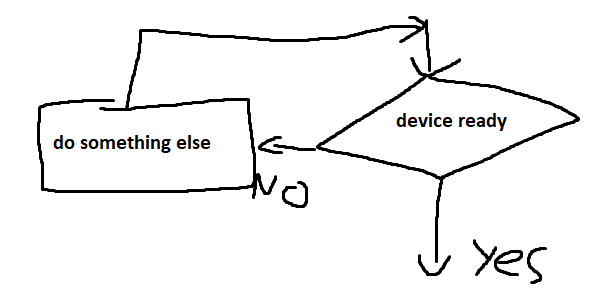
\includegraphics[width = 80mm]{IO.PNG}
    \caption{Polling}
    \label{fig:my_label}
\end{figure}
\newpage

\section{Contrast busy-wait and interleaved polling. Your answer should use labelled diagrams where appropriate.}
busy-wait polling is where we read the status of an IO device and if it is not
ready we just read the status again on repeat until its ready.

\begin{figure}[h]
    \centering
    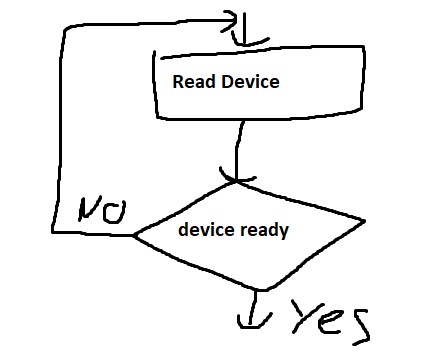
\includegraphics[width = 80mm]{IO3.PNG}
    \caption{busy-wait polling}
    \label{fig:my_label}
\end{figure}

Interleaved polling is similar but instead of just repeatedly checking whether
the device is ready, we do another task while waiting for the device to be
ready. This allows for better multi-tasking.
\begin{figure}[h]
    \centering
    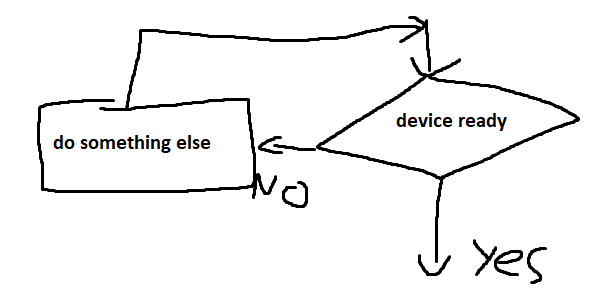
\includegraphics[width = 80mm]{IO.PNG}
    \caption{interleaved polling}
    \label{fig:my_label}
\end{figure}

\section{Discuss the advantages and disadvantages of polling}
advantages:\\
Simple software and hardware required to perform polling. Need a looping
construct for software and a notion of "ready" for hardware.\\
disadvantages:\\
A lot of CPU time and power is wasted on checking IO devices.\\
Also, interleaving tasks can lead to a significantly delayed response to a
device.

\section{Explain, using appropriate diagrams, how interrupts can be used to provide asynchronous IO}
\begin{figure}[h]
    \centering
    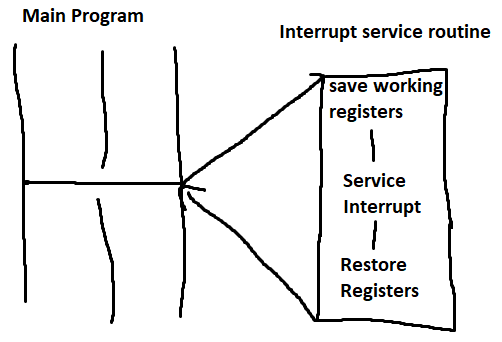
\includegraphics[width = 80mm]{IO2.PNG}
    \caption{Interrupt}
    \label{fig:my_label}
\end{figure}

The figure above shows how when an interrupt is called a Jump is made to a
service routines which is performed before going back to the main program.\\
These interrupts forces the CPU to jump between service routines which can make
it appear that the CPU is performing 2 or more tasks "simultaneously"

\section{Explain context switching}

when an interrupt is called the CPU completes its current instruction then
pushes the PC and SR's to a stack.\\
Then load the PC with the address of the Interrupt Handler.\\\\
When returning from an Interrrupt we pop the PC and SR's from the stack then
load the PC with the popped return addresses.

\section{Discuss the advantages and disadvantages of interrupts as a mechanism for IO}
Advantages:\\
Fast response\\
No wasted CPU time\\\\
Disadvantages:\\
All data trannsfer is controlled by the CPU\\
complex hardware and software.

\section{Contrast the suitability of polling and interrupt driven IO for use in an embedded system of your choice. Your answer should state any assumptions clearly}
Chosen embedded system - A safety critical system for an airplane.\\
For a device like this polling would be detrimental as there will be a lot of
time where we are checking whether an IO device is ready to respond instead of
performing the safety-critical operation. This means that there is a lot of time
where the CPU is not performing its operation.\\
Interrupts are much better suited for a safety critical system. This is because
a lot less time is wasted on checking whether IO devices are ready to be used.
This means there is a fast response which is needed for safety-critical systems

\section{Explain Direct Memory Access (DMA). Your answer should give an example of where DMA would be a suitable choice as an I/O mechanism.}

DMA is where the use of system busses is surrendered by the CPU to a DMA
Controller (DMAC). This avoids the bottleneck of the CPU for I/O.\\
When an IO device needs to access the system busses they request a DMA transfer,
the DMAC passes the request to the CPU. Then the CPU initialises DMAC which
requests use of system buses. The CPU then responds with a DMA Ack when it's
ready to surrender buses.\\
There are 2 modes of operations for DMA: cycle stealing and Burst Mode.\\
Cycle stealing is where the DMAC uses system busses when they are not being used
by the CPU.\\
Burst mode is where the DMAC requires system buses for extended transfer of
large amounts of data. The DMAC locks the CPU out of using the system buses for
a fixed time or until the CPU received an interrupt from a greater priority.
\newpage







\end{document}
